% Chapter Experiment

\chapter{Experimental Setup at the IP2I cryogenic facility} % Main chapter title

\label{ChapterExperiment} % Change X to a consecutive number; for referencing this chapter elsewhere, use \ref{ChapterX}

%----------------------------------------------------------------------------------------
%	BEGING CHAPTER
%----------------------------------------------------------------------------------------

This chapter describes the IP2I Cyostat Facility in which the cryogenic germanium detectors presented in this work were operated. It explains how cryogenic conditions are obtained, presents the cryogenic germanium detectors and their principle of operation.

\section{The IP2I cryogenic facility}
\label{sec:IP2I-cryostat-facility} 

% Intro
The particles detectors studies in this work are cryogenic germanium bolometers. The term "cryogenic" indicates that these detectors are operated at cryogenic temperatures below $\SI{1}{\kelvin} = \SI{-272,15}{\celsius}$. In order to reach such temperatures, the detectors are placed inside of a cryostat.

The experimental results discussed in this work were obtained by running germanium detectors in the the dry dilution cryostat of the \textit{Institut de Physique des 2 Infinis de Lyon} (IP2I). The IP2I cryogenic facility is located in the basement of the IP2I Haefely building (see figure \ref{fig:haefely-building}). With an almost negligible overburden roughly estimated to be about \SI{1.5}{m.w.e}, the cryogenic detectors are operated in an above-ground or surface experiment as opposed to the underground operation of the EDELWEISS detectors at the LSM.

% Radioactive shielding
In order to reduced the environmental gamma background, the cryostat is surrounded by a \SI{10}{\cm} thick cylindrical lead shield covering a solid angle of $\sim \SI{70}{\percent}$ of $4\pi$ around the detector. A reduction of about a factor of 10 is estimated on the triggering rate of our detectors with this lead shield.
There is no lead shield inside the cryostat. The materials used for the cryostat construction were not selected for low radioactivity, with the exception of the replacement of the standard glass fiber rods used by Cryoconcept by stainless steel ones, shown to have much less radioactive contamination. 
While the radioactive background is high as a consequence of the above-ground operation, it is very similar to what is expected from the ILL site for the \Ricochet{} experiment. The neutron and gamma components of this background are characterized down to \SI{1}{\kilo\eV} in the Chapter \ref{ChapterNeutron}.

\begin{figure}
\centering
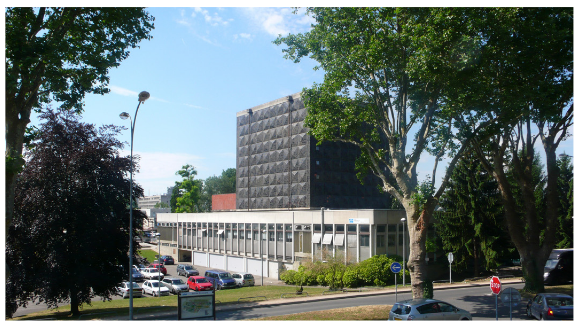
\includegraphics[width=\textwidth,angle=0]{Figures/Experiment/haefely_building.png}
\caption{Photo of the IP2I Haefely building. The cryogenic facility is located in the basement, at the same height as the parking lot.}
\label{fig:haefely-building}
\end{figure}

The total surface area of the facility is about a \SI{100}{\m^2} and encompasses the main cryogenic lab (\SI{80}{\m^2}), a technical room for pumps and gas handling system (\SI{6}{\m^2}), an ISO-5 clean room for detector mounting (\SI{9}{\m^2}), and a room hosting a chemical bench also related to detector fabrication (\SI{5}{\m^2}). A photo of the cryogenic laboratory is displayed in figure \ref{fig:cryolab} with the open cryostat in the corner of the room next to the lead shielding of the left and the acquisition electronics and computers on the right.

\begin{figure}
\begin{center}
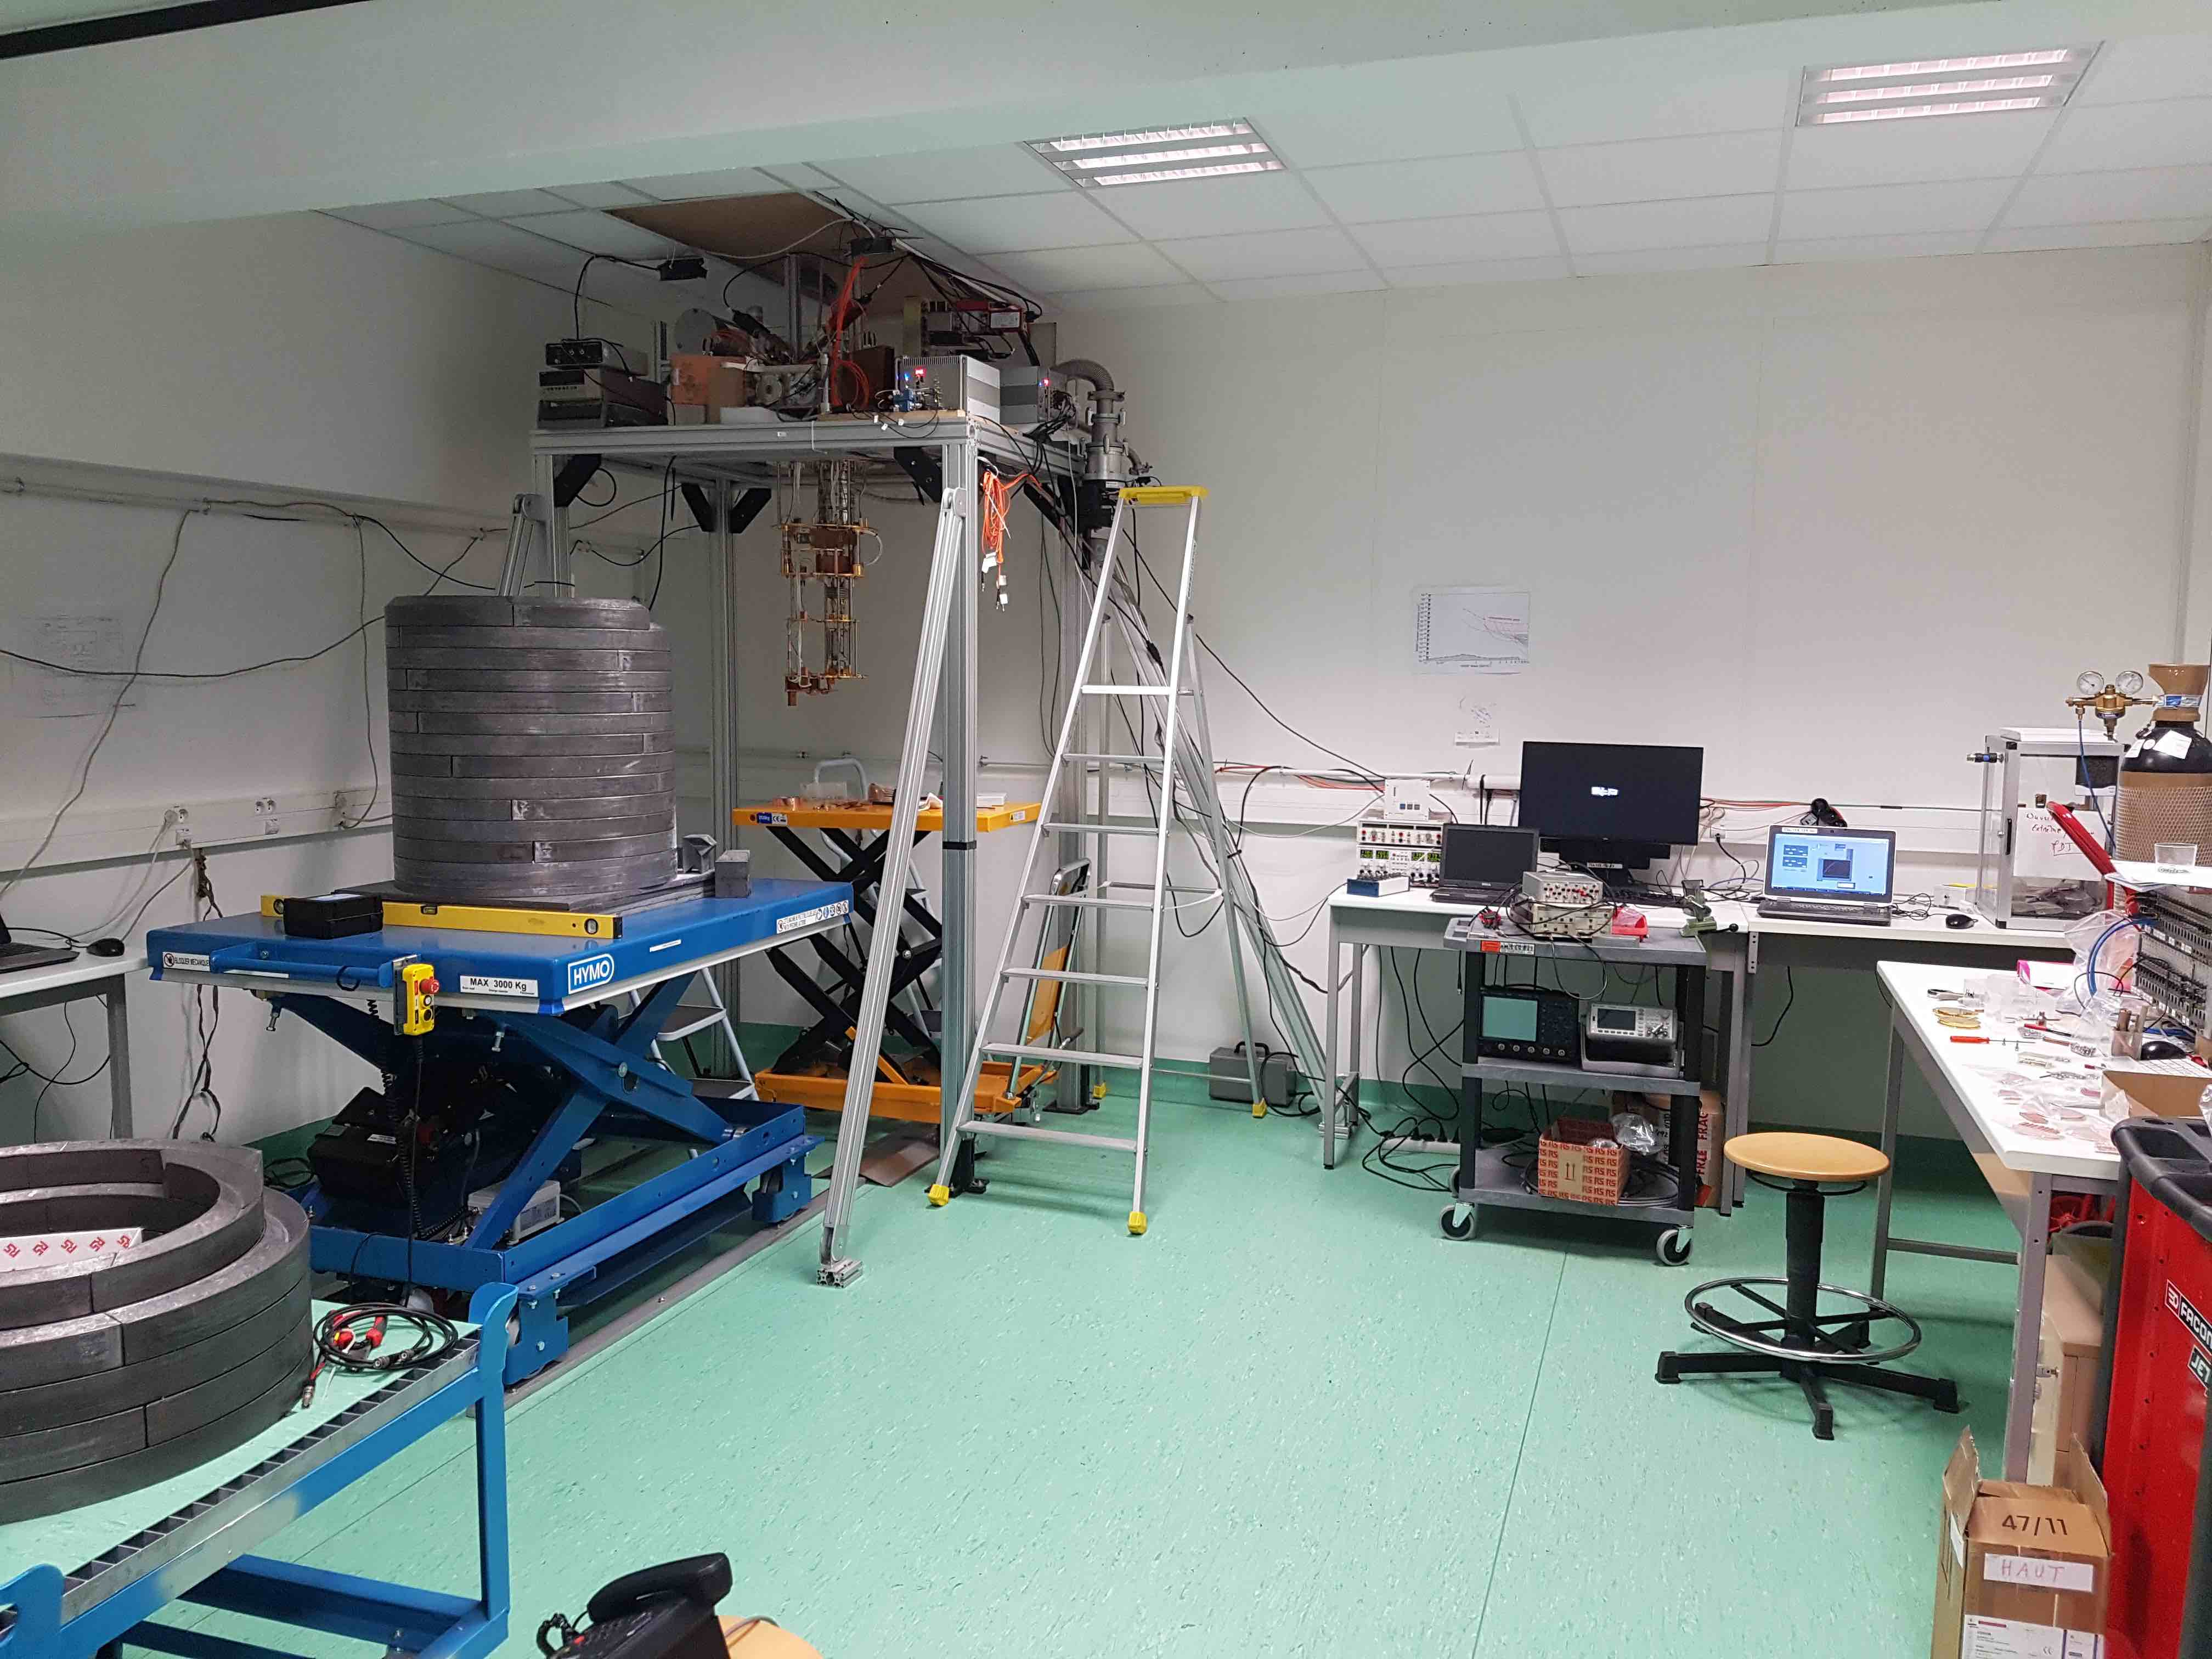
\includegraphics[width=\textwidth,angle=0]{Figures/Experiment/ip2i_cryogenic_facility.jpg}
\caption{Photo of the cryogenic lab, where the dry dilution cryostat (opened) and its lead shield are clearly visible. On the left side are the computers controlling the cryostat, and on the right side are the computers and outside electronics in charge of the detector readout and polarization.}
\label{fig:cryolab}
\end{center}
\end{figure}

\subsection{Presentation of the IP2I R\&D Dry Cryostat}

% Cryostat intro
The cryostat is a Hexadry-200 commercially available from Cryoconcept, which has been upgraded to reduce the vibration levels on the mixing chamber.
The cryostat assures a cryogenic temperature with low fluctuations and a temperature setpoint of about \SI{20}{\milli\kelvin} on the bolometers. It provides a steady cooling power over several weeks for standard R\&D runs which can be extended to several months for physic runs.

% Cryostat structure
The structure of the cryostat is illustrated with annotated photo and scheme displayed in the figure \ref{fig:cryo-photo}. This cryostat is built with several cooling stages at different temperatures which allow the transition from the exterior ambient temperature $\sim \SI{300}{\kelvin}$ to the lowest cryogenic temperature $\sim \SI{10}{\milli\kelvin}$ on the mixing chamber. During operation, the cryostat is maintained hermetically shut with the Outer Volume Casing (OVC) mounted on the feedtrough of the cryostat. The whole inner volume is immersed in a medium vacuum, the air is pumped out to reach a pressure less than \SI{e-3}{\milli\bar}). As such, there is no atmosphere to conduct heat between the different stages. The thermal conduction between stages can only occur though the metal structure of the cryostat, the cooling circuit and the thermal radiation. Each stage is surrounded by gold-plated copper casings to block the infrared radiation of black body type.

\begin{figure}
\centering
\begin{minipage}{0.48\textwidth}
	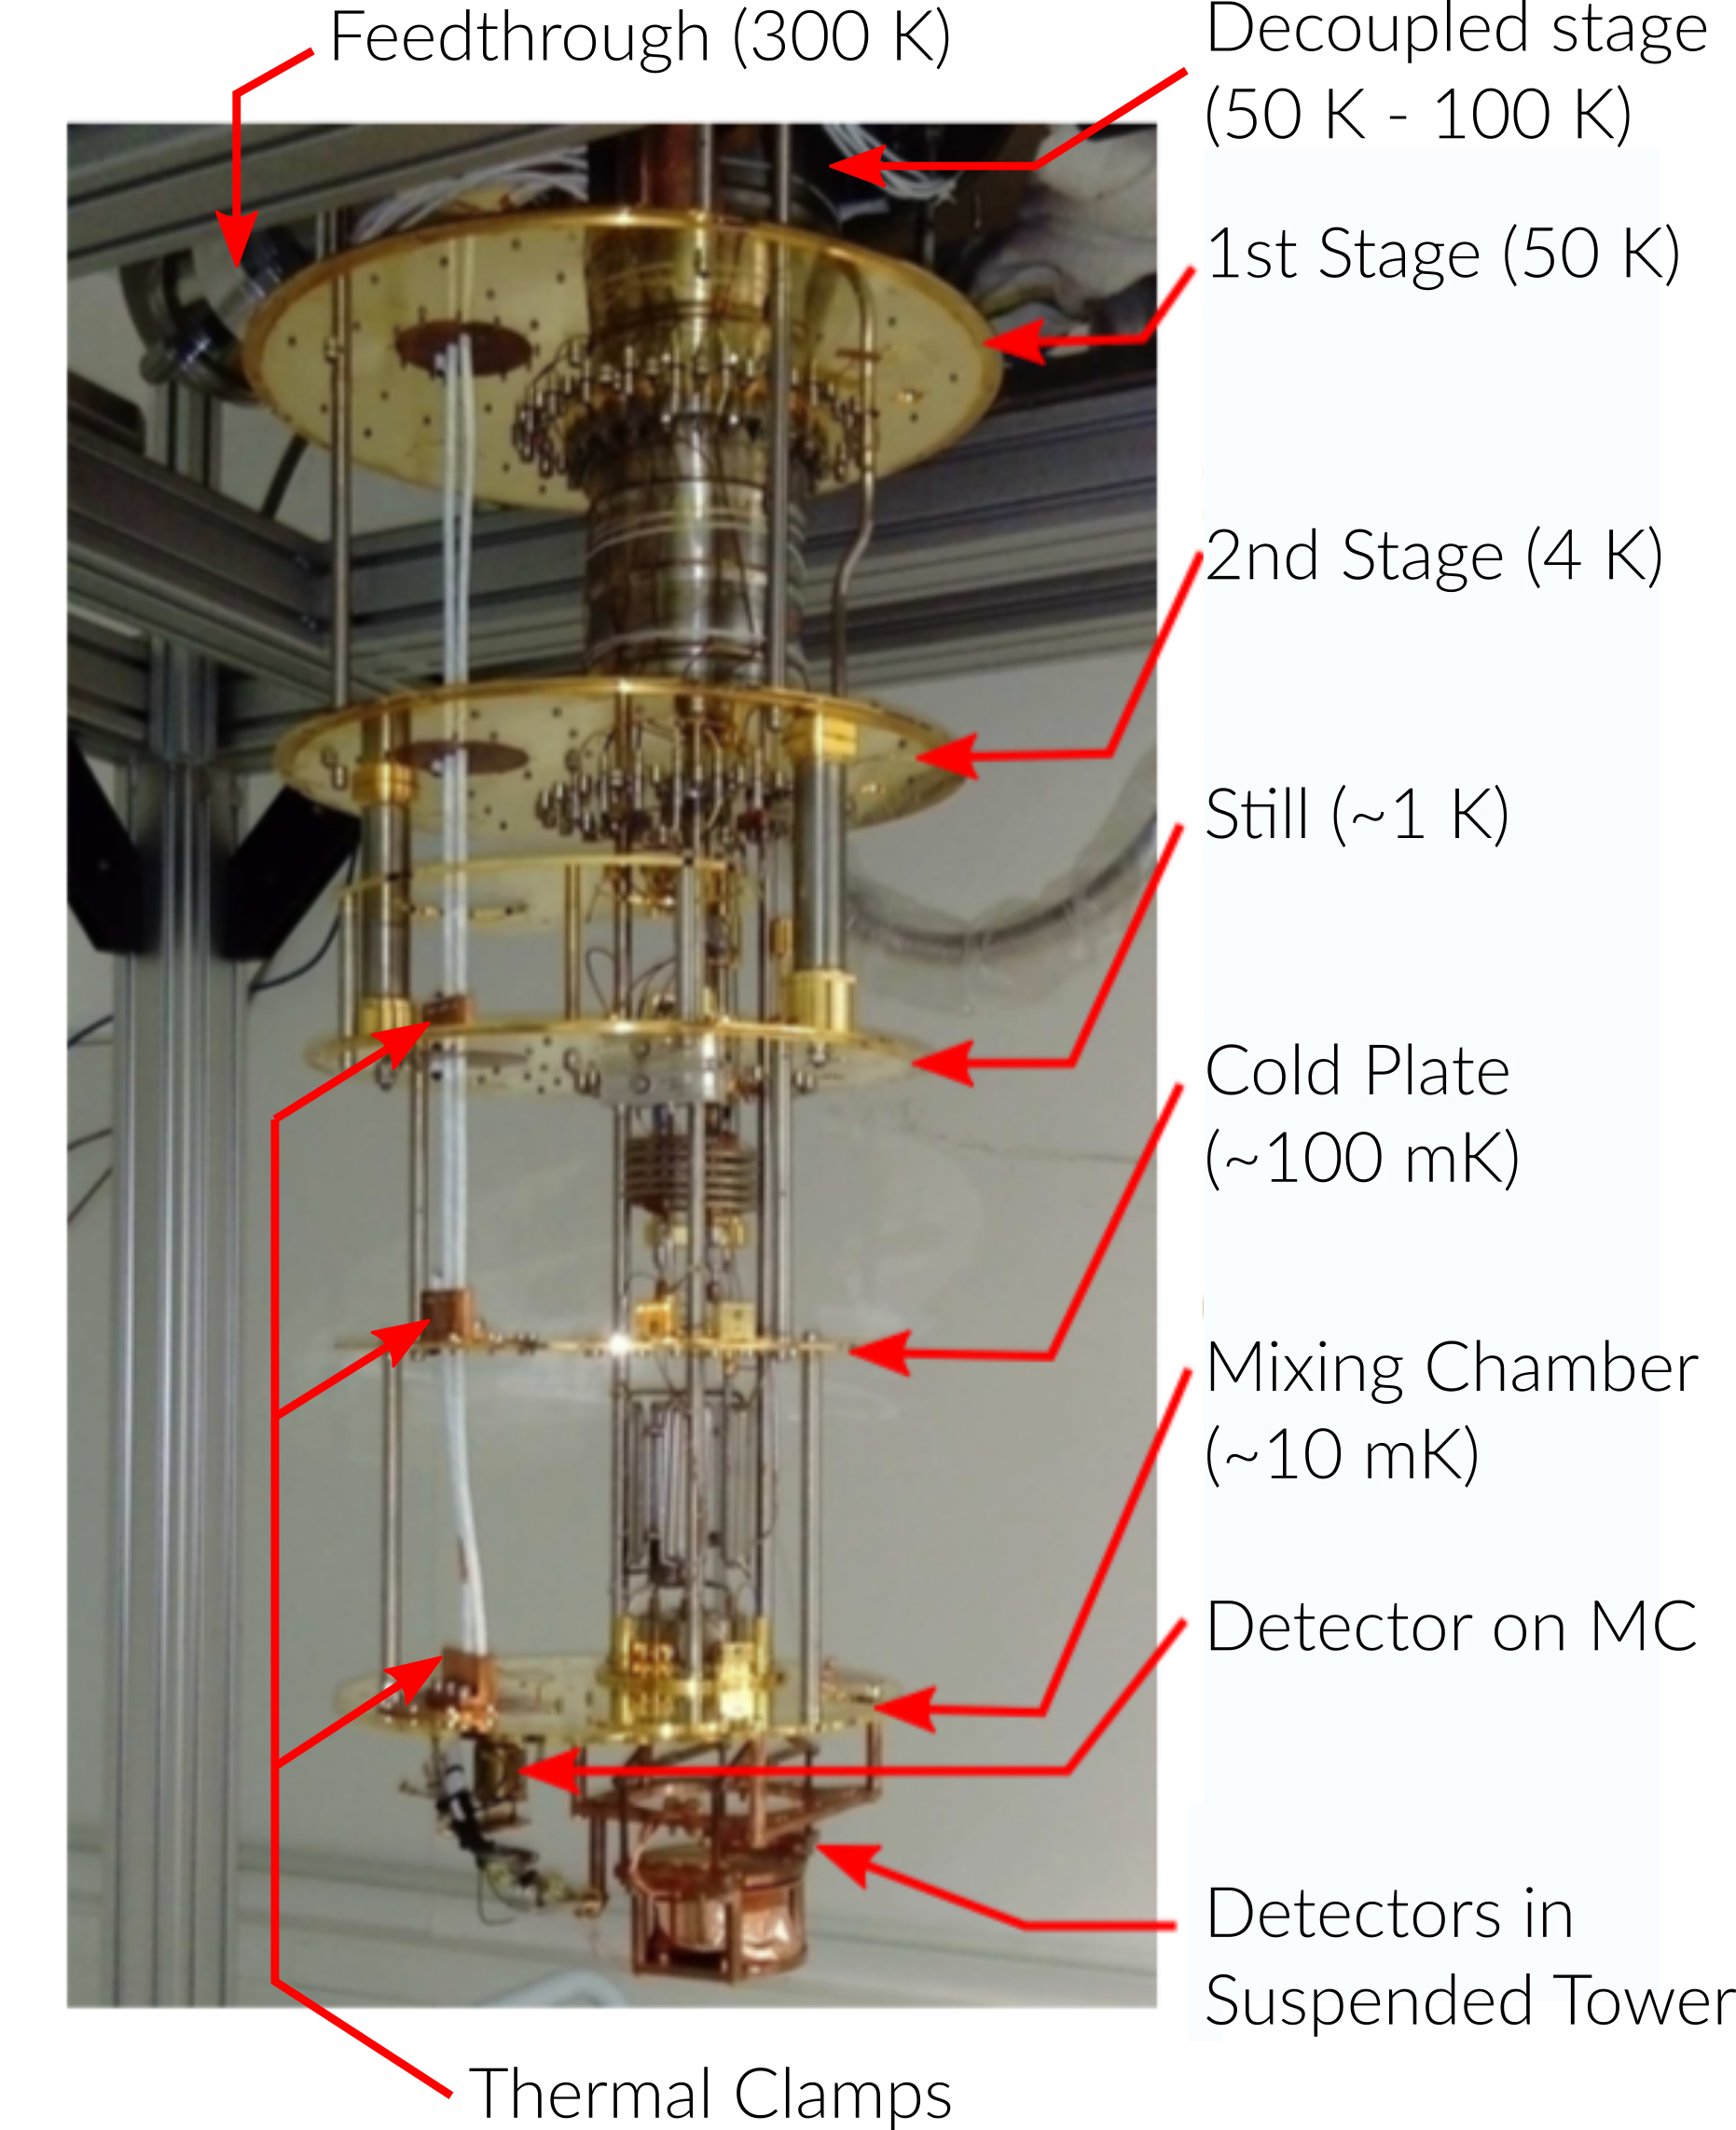
\includegraphics[width=\textwidth]{Figures/Experiment/cryo_photo.png}
\end{minipage}
\hfill
\begin{minipage}{0.48\textwidth}
	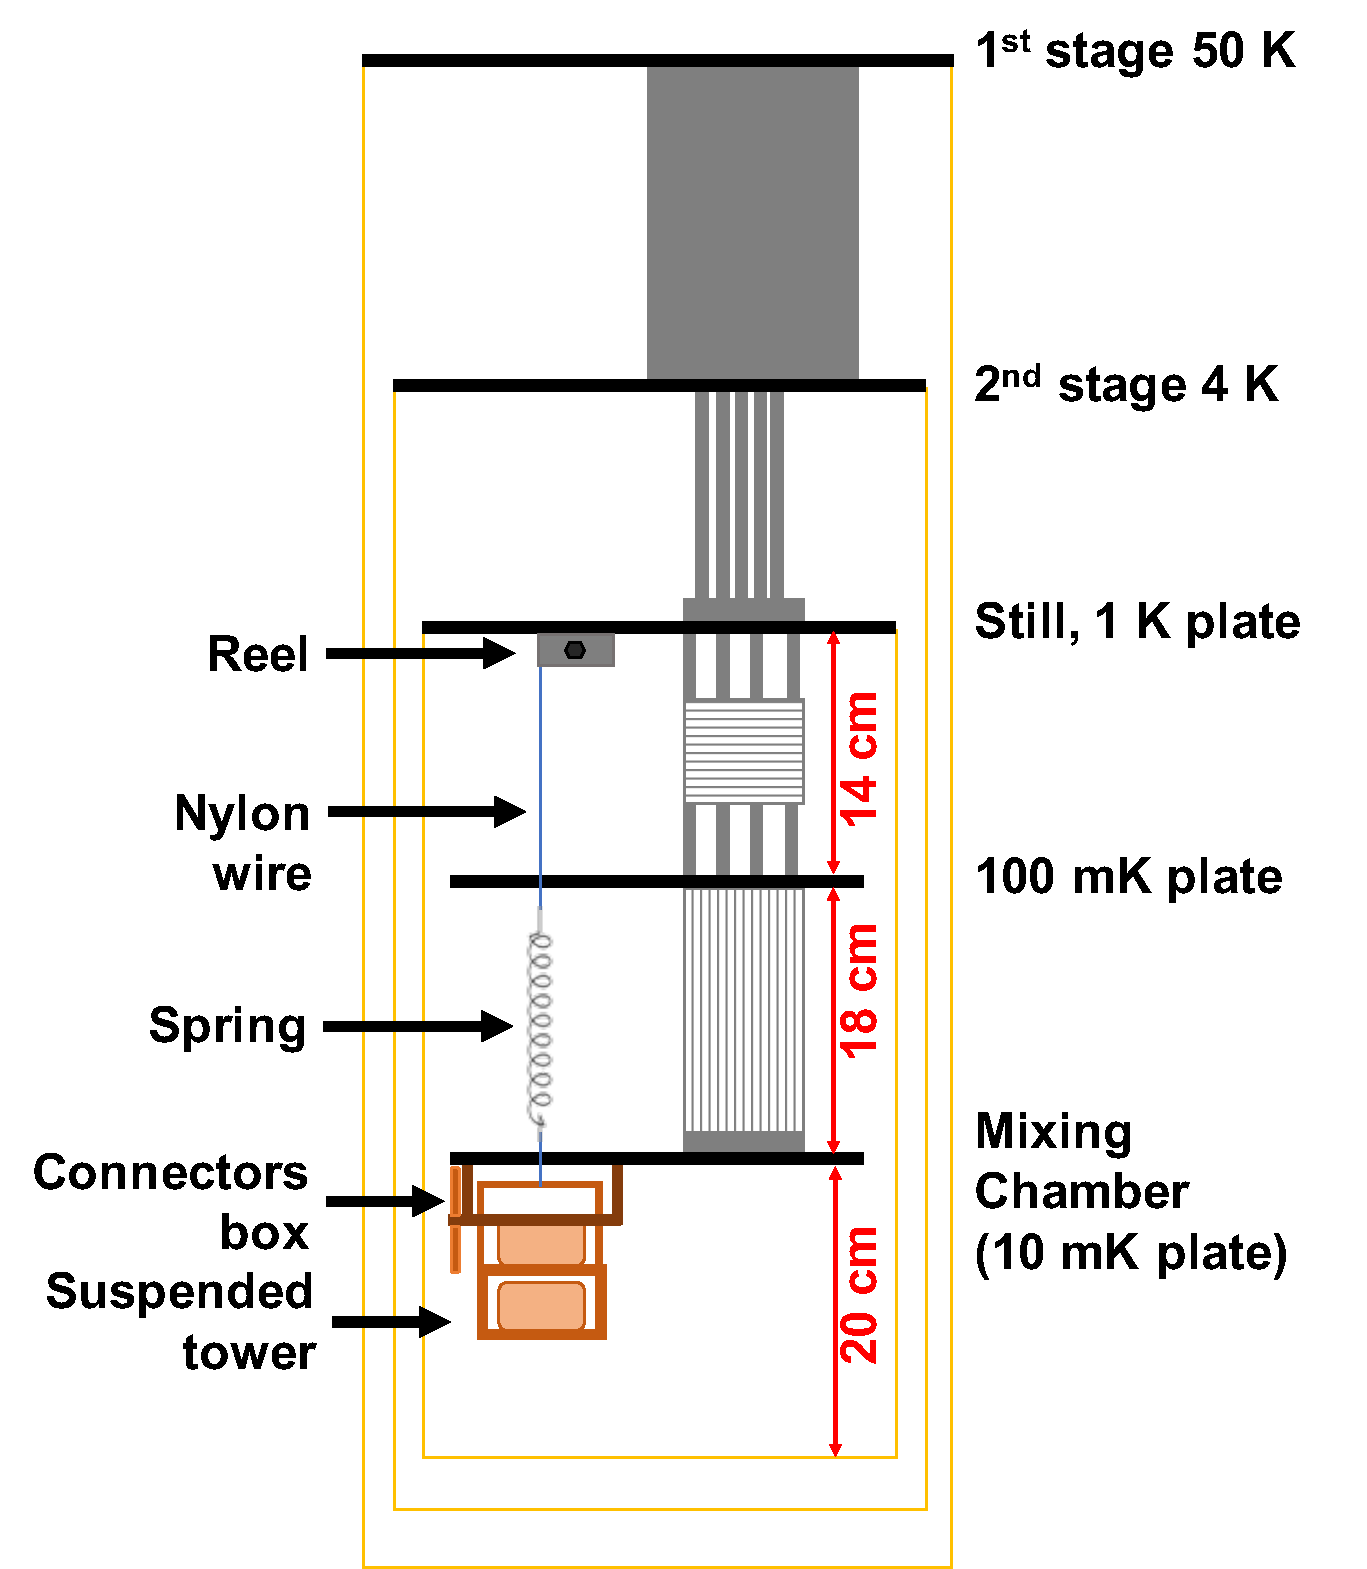
\includegraphics[width=\textwidth]{Figures/Experiment/cryo_sketch.pdf}
\end{minipage}
\caption{On the left, annotated photo of the open cryostat. On the right, annotated scheme of the cryostat. The copper screens blocking the infrared radiations are represented as the orange rectangles separating each cooling stage.}
\label{fig:cryo-photo} 
\end{figure}

% Dry cryostat
The IP2I cryostat is a Dry Dilution Refrigerators (DDR) the dry dilution cryogenic cooling technology. It runs solely on electric power as opposed to the Wet Dilution Refrigerators (WDR) of the EDELWEISS experiment which consumes liquid helium to cool down. Dry cryostats are particularly adapted to R\&D work as the operating cost are low and it is possible to descend very quickly to cryogenic temperatures (24 hours to reach \SI{4}{\kelvin}, compared to one week for the EDLWEISS cryostat at the LSM). They provides a similar low temperature environment as the one obtained with WDR at the cost of increased vibration levels. The IP2I cryostat was equipped with vibration mitigation solutions described in the next section \ref{sec:suspended-tower}.

% Cooling circuit
The IP2I dry cryostat has one closed cooling circuit using as cooling fluid a mixture of \ce{^4He} and \SI{25}{\percent} \ce{^3He}. This cooling circuit is separated in two cycles: the "Pulse Tube" cycle and the dilution cycle. 
% Pulse tube cycle
The pulse tube cycle is in charge of cooling the first stage and second stage to reach the temperatures \SI{50}{\kelvin} and \SI{4}{\kelvin} respectively. The "Pulse Tube" applies Stirling cycles between 9 and 18 bars at a frequency of \SI{1.6}{\Hz}, which allows the \ce{{}^4He} fluid to reach a temperature of \SI{4}{\milli\kelvin}.
% The dilution cycle
The dilution cycle extends the cooling circuit to the three other stages and cools them to their operating temperatures: the still at \SI{1}{\kelvin}, the cold plate at $\sim \SI{100}{\milli\kelvin}$ and the mixing chamber (MC) at $\sim \SI{10}{\milli\kelvin}$. In this cycle, the helium mixture is cooled by passing through fine capillaries located on the first and second stages, benefiting from the cooling of the pulse tube cycle. As the cooling fluid reaches \SI{4}{\milli\kelvin}, it condensates in its liquid phase. A succession of Joule-Thompson expansion valves and heat exchangers allows the mixture to reach a temperature of \SI{800}{\milli\kelvin} at the still. It is near this temperature that a phase separation occurs within the mixture: the first phase is concentrated in \ce{{}^3He} and floats on the surface of the second phase diluted in \ce{{}^3He} and rich in \ce{{}^4He}. This phenomenon can be explained by the Fermi-Dirac statistic followed by the \ce{{}^3He} atoms: they cannot simultaneously occupy the same energy state and the same position. Thus, for a sufficiently low temperature, the phase separation becomes energetically favorable. This phase separation takes place within the mixing chamber. The phase with low \ce{{}^3He} is then pumped out. The thermodynamic equilibrium of the two phases is broken and there is a transfer of \ce{{}^3He} from the concentrated phase to the diluted phase in \ce{{}^3He}. This process is endothermic, which decreases the temperature of the mixture and thus of the mixing chamber. The pumped helium \ce{{}^3He} is then re-injected into the dilution circuit. In this end, the dilution cycle allows a minimum temperature of \SI{9}{\milli\kelvin} to be reached on the mixing chamber for this cryostat. The detector load thermally linked to the mixing chamber in order to reach the lowest temperatures and the best performances.

% Thermal regulation
Once the cryostat is cooled down, it continues to operate at full power until the end of the run. The power of the cooling circuit is in constant equilibrium with the thermal heat coming from the exterior of the cryostat or from the operation of the detectors. Consequently, in this state, the exact temperature of the mixing chamber would fluctuates near its minimal equilibrium value. 
As a mean to operate the cryogenic detectors with constant performances at a chosen temperature order to stabilize, the temperature of the mixing chamber is regulated at higher temperatures usually superior to \SI{14}{\milli\kelvin}. The regulation is assured by the Joule effect of heating resistor. Its heat power is set by a Proportional-Integrate-Derivative controller (PID controller) reading the temperature with an \ce{RuO_2} thermistance close to the detectors suspended tower to choose exactly their operating temperature.


\subsection{Standard Operation of the Detectors}

% detector load and electronics
We want to operate the bolometers at the coldest temperature possible. We may want to attach the detectors directly on the mixing chamber stage as seen on left photo of figure \ref{fig:cryo-photo}. However, the "dry" cryostat creates a lot of mechanical vibration especially due to the pulse tube cycle. These vibrations propagate to the detectors, causing thermal noise (parasitic phonons), electric noise (triboelectricity) as well as heat power on the mixing chamber which prevents a good cooldown.
% cite{Olivieri:2017lqz}
To tackle this issue, the cryostat is mechanically decoupled from the ceiling/pulse tube with a bellow (external decoupling). This external decoupling was done in partnership with Cryoconcept by mechanically decoupling the cold head of the pulse tube cryocooler from the dilution unit. The vibrations at the detector level were further mitigated by placing the bolometers inside a suspended tower (internal decoupling) developed by the Manoir group.
%\cite{romain}
The suspended tower is a copper chassis solely linked to the cryostat by a spring providing mechanical support and mechanical decoupling. This device makes it possible to avoid a significant low-frequency noise on the heat measurement while ensuring thermal conduction to the cryostat thanks to thin copper braids. This suspended tower is described in the paragraph \ref{sec:suspended-tower}.
% \cite{Maisonobe:2018tbq}

The detectors are cabled to the acquisition computer on the outside of the cryostat through the cold and warm electronics. The cold electronics function is transport the voltage signal of the detectors located near the mixing chamber to a first Bi-FET preamplifier stage at 100 K and a second stage amplifier at 300 K.
% ~\cite{Armengaud:2017rzu}
The white cables of this cold electronic are visible on the left photo of figure \ref{fig:cryo-photo}. The cabling comes from the top of the cryostat and goes down thermalizing at each stage with the thermal clamps. As such, only there is only minimal heat transfer from the hotter stages  on the mixing chamber due to the electronics.
Once the signal is amplified, it is transported to the acquisition computer with optic fiber. The detector signals are recorded as continuous time series called data streams. These data streams are then processed with a dedicated pipeline based on the NEPAL software developed by the Manoir group in order to ensure high quality data processing. The stream processing and analysis is described in the chapter \ref{ChapterElectrodesExperimental}. Once the processing is done at the CC-IN2P3, monitoring plots are transferred automatically to a monitoring website allowing us to follow the performance and behavior of the detectors as a function of time.

%%% Bonus
%% IP2I Cryostat for Ricochet 
%By early 2021, our cryogenic lab will be hosting the \Ricochet{} cryostat for a little over one year in order to be fully commissioned prior to its deployment at ILL. The commissioning phase includes: validation of the cabling (noise and thermal performance), the cold front-end electronics, the cool down of the inner shielding layers (lead and polyethylene), the demonstration of the CryoCube detector array performance (threshold, particle identification capability and livetime), and the DAQ and monitoring pipelines.


\section{Vibration mitigation and cryogenic suspension}
\label{sec:suspended-tower}

% Motivation
The cool-down process of the two first stages within DDR is ensured by the technology of pulse-tube cryocoolers. However, the mechanical vibrations they induce can drastically affect the performance of cryogenic detectors. This effect has been reported by several cryogenic experiments using such bolometers.
%\cite{Caparrelli:2006zkj,Haan:2013iwa,Olivieri:2017lqz}. 

% external mitigation
The IP2I cryostat was upgraded with an external vibration mitigation solution. Its first two stages (50K and 4K) are thermally coupled to the highly vibrating pulse-tube cold head thanks to low-pressure gas exchangers (Hexagas$^{\rm TM}$), hence avoiding any mechanical contact and vibration propagation to the dilution unit. In 2016, one year after its delivery to IP2I, the cold head has been mechanically anchored to the ceiling hence providing two independent and maximally decoupled frames. In the figure \ref{fig:cryolab}, the metallic framework surrounding the cryostat supports and anchors the dilution unit to the ground, while the cold-head is fixed in the ceiling of the laboratory (hidden by a wooden panel on the photo).

% results
This upgrade lead to the reduction of the vibration levels by about two orders of magnitude between \SI{0.5}{\Hz} and \SI{20}{\Hz} hence achieving world-leading vibration levels in a dry cryostat of few-\si{\micro g \per \sqrthz}.
 %below 20-Hz~\cite{Olivieri:2017lqz}.
At the time, the impact on our detectors has been tremendous. Indeed, before the decoupling, due to the high vibration levels, the detectors were not able to operate due to the significant vibration-induced  frictional heat power dissipation. 

% Motivation internal
% External Mitigation results 
With the improvement of our detector sensitivity and resolution, we found that the cold-head decoupling was not enough to ensure optimal operation of the new generation of detectors. Indeed, it was found that the large radial stiffness of the edge-welded below connecting the cold-head to the dilution unit still allows for some vibration propagation down to the detectors. A second vibration mitigation system at the mixing chamber level, where the detectors are installed, had to be implemented.


\subsection{Internal Mitigation Solution: the Suspended Tower}

%% Internal mitigation
%This internal vibration mitigation is the suspended tower presented in the annotated photo \ref{fig:suspended-tower}. This device consists in a 25 cm long elastic pendulum, attached to the \SI{1}{\kelvin} stage by a Kevlar string and a stainless steel spring with an elastic constant of \SI{240}{\newton\per\meter}, holding the detector tower situated below the mixing chamber at \SI{10}{\milli\kelvin}. The detector tower is thermally anchored to an intermediate safety structure via supple copper braids. This safety structure also hosts the connectors for the detector readout.

% suspended tower theory
This internal vibration mitigation solution is the suspended tower. A detector placed in this device can be considered mechanically as a simple elastic pendulum.
The 3-D dynamical description of the elastic-pendulum can be divided into two pseudo-independent equations in the approximation of small perturbations. The natural frequency for vertical modes is then given by:
\begin{equation}
f_{0,\textrm{vertical}}=\frac{1}{2\pi}\cdot\sqrt{\frac{k}{M}} = \frac{1}{2\pi}\cdot\sqrt{\frac{g}{(l_{\textrm{eq}}-l_{0})}}\label{eq:Freq-Vertical},
\end{equation}
where $M$ corresponds to the total mass of the suspended tower, $k$, $l_0$, and $l_{\rm eq}$ are the elastic constant, the rest length, and the length at equilibrium of the spring, respectively. The vertical resonance frequency can either be expressed of $k$ and $M$ simultaneously or by its elongation length alone $|l_{\textrm{eq}}-l_{0}|$. The natural frequency for radial oscillations of the pendulum, which are related to its total length  $l_{\rm tot}$, is given by:
\begin{equation}
f_{0,\textrm{ radial}}=\frac{1}{2\pi}\cdot\sqrt{\frac{g}{l_{\rm tot}}}\label{eq:Freq-Radial}.
\end{equation}
From these approximations, we can estimate the theoretical resonance frequencies of the elastic pendulum depending on the spring constant, the pendulum length and the total mass of the detector assembly. Interestingly, one can notice that as $l_{\textrm{tot}} \geq (l_{\textrm{eq}}-l_{0})$, the natural frequency in the radial direction is necessarily lower than in the vertical direction: $f_{0,\textrm{ radial}}<f_{0,\textrm{vertical}}$. 

Thanks to the use of a single spring holding system, we avoid any transverse momentum related natural frequencies which could populate the vibration spectrum at high frequencies. Therefore, system is expected to have a transfer function response under the form of a 2\textsuperscript{nd} order low-pass filter with a single resonance frequency in both directions $i=\left\{ \textrm{vertical, radial}\right\}$:
\begin{equation}
H(\omega_{i})=\frac{\omega_{0,i}^{2}}{\omega_{0,i}^{2}-\omega_{i}^{2}}\label{eq:Transfer-function},
\end{equation}
where $\omega_{0,i}$ is the natural pulsation of the suspended tower, with $\omega_{0,i}=2\pi\cdot f_{0,i}$. 
The natural frequencies of the suspended tower in both vertical and radial directions have been tuned to be as low as possible in order to attenuate all vibrations above \SI{1.4}{\Hz}, corresponding to the frequency of the pulse-tube cryocooler. According to equation \ref{eq:Freq-Vertical}, we obtain a vertical resonance frequency $f_{0,\textrm{vertical}} \leq \SI{1}{\Hz}$ for a spring elongation of at least $(l_{\textrm{eq}}-l_{0})\geq \SI{25}{\cm}$. The same condition applied to the radial frequency, $f_{0,\textrm{radial}} \leq \SI{1}{\Hz}$ results in a total pendulum length of at least  $l_{tot}\geq \SI{25}{\cm}$ using equation \ref{eq:Freq-Radial}.

The challenge then comes from accommodating with the constraints imposed by the cryostat geometry. As the distance between the mixing chamber plate and the inner thermal screen is only of about \SI{20}{\cm}, the pendulum had to be attached to the still plate and not directly to the mixing chamber.
The scheme of the figure \ref{fig:cryo-photo} and the photo \ref{fig:suspended-tower} illustrate the holding strategy of the suspended tower in the cryostat. 
A Kevlar wire is fixed below the still plate at \SI{1}{\kelvin} and running without contact through the cold plate at \SI{100}{\milli\kelvin}. 
A stainless steel spring with an elastic constant of $k=\SI{240}{\newton\per\meter}$ is attached to the wire between the cold plate and the MC at \SI{10}{\milli\kelvin}. The elastic constant $k$ has to be carefully chosen, taking into account the total mass of the detector assembly $M$, as its elongation is constrained by the $\sim \SI{18}{\cm}$ distance between the \SI{100}{\milli\kelvin} stage and the MC. 
Finally, the suspended tower is connected to the spring via a thick ($\sim \SI{2}{\mm}$ in diameter) \SI{5}{\cm} long copper wire through the MC plate. This copper wire ensures the thermalization of the stainless steel spring. so that it does not emit infrared radiation damaging the detector performance.
With this approach, the total pendulum length from the still plate to the center of mass of the detector assembly is $l_{\textrm{tot}} = \SI{25}{\cm}$.


\begin{figure}
\centering
\captionsetup{justification=centering}
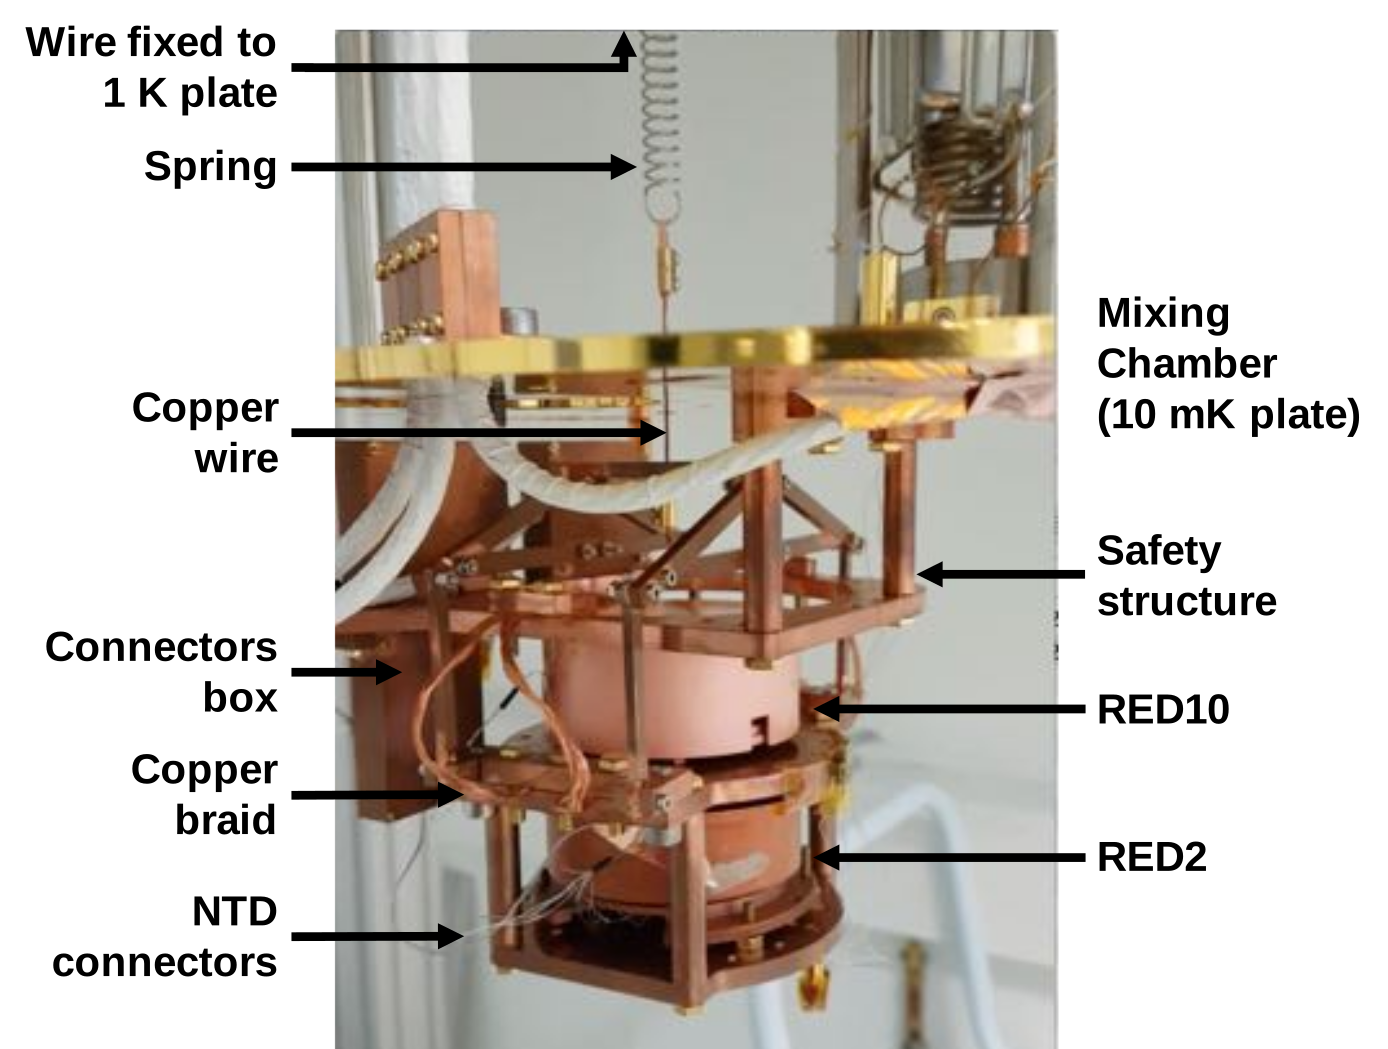
\includegraphics[height=9cm]{graphics/damocles.png}
\caption{Photo of the suspended tower containing the two $\SI{200}{\g}$ bolometers RED10 and RED2. This device mechanically decouples the detector load from the mixing chamber while assuring its thermalization.}
\label{fig:suspended-tower} 
\end{figure}

The detector tower is shown in the right panel of Fig\ref{fig:suspended-tower} holding the two detectors RED2 and RED10 . This module has a total height of \SI{13}{\cm} and can hold two cryogenic detectors based on \SI{200}{\g} germanium crystal or lighter. During the installation, before attaching the spring, the tower is firmly held by a copper frame screwed under the MC plate. This structure remains as a safety structure during cool-down and operation in case the wire should break. Connector boxes are placed close to the detector on the external side of the safety structure. They are used to connect the sensors of the detectors to the readout electronics at the warmer stages. Both the suspended tower and the safety structure are made of clean \ce{CuC_2} copper. During operation, the suspended tower is floating and its thermalization is realized by four \SI{10}{\cm} long ultra-supple flat copper braids linking the safety structure and the tower.


\subsection{Characterization of the Vibration Levels}

This subsection quickly presents the impact of the suspended tower on the vibration level and the noise of the heat channel of the bolometer RED10. All the results are published in the paper \cite{Maisonobe:2018tbq} in which the suspended tower was demonstrated to attenuate the transmission of both vertical and radial vibration, with a particular emphasis on the radial modes as these are less efficiently damped from our pulse-tube cold head decoupling. 

The vibration level is characterized by measuring the movement of the detectors.
%\cite{Olivieri:2017lqz}
The set-up is composed of a high sensitivity seismic accelerometer from \emph{PCB Piezotronics}. We used the high sensitivity accelerometer \emph{PCB-393B05} which has a gain of \SI{10}{\volt\per g} and an intrinsic noise limit of $\textrm{[0.5-0.07]}\,\textrm{g}/\sqrt{\textrm{Hz}}$ within $\textrm{[1-1000]}\,\si{\Hz}$ frequency range.

The accelerometer is fixed on U-shaped workpiece allowing to measure the vibrations along either the radial or the vertical direction.  The accelerometer can be fixed below the MC stage of the cryostat, or below the bottom stage of the suspended tower in order to compare their respective vibration level. 
The elastic constant $k$ and Young's modulus $E$ values of the stainless steel and copper, composing the majority of the rigid strucutre of the cryostat, have small variation between ambient and cryogenic temperature. As such, all vibration measurements are performed at room temperature.
%~\cite{Emodulus}.
The output signal of the accelerometer is sampled at \SI{10}{\kilo\Hz}, well beyond the signal bandwidth of the accelerometer of \SI{1}{\kilo\Hz}. The vibration levels is obtained as LPSD expressed in \si{g \per \sqrthz} from a Fast Fourier Transform (FFT) analysis using Hanning windowing over \SI{5}{\s} time windows.
Figure~\ref{fig:Status-Tower-vibrations-PTonoff} displays the vibration levels on the MC plate and in the suspended tower comparing the measurements with the pulse-tube (PT) cryocooler switched on (PT ON), emulating the normal cryostat operation, or off (PT OFF). The intrinsic noise limit of the accelerometer is plotted as dashed lines as reference.

\begin{figure}
\centering 
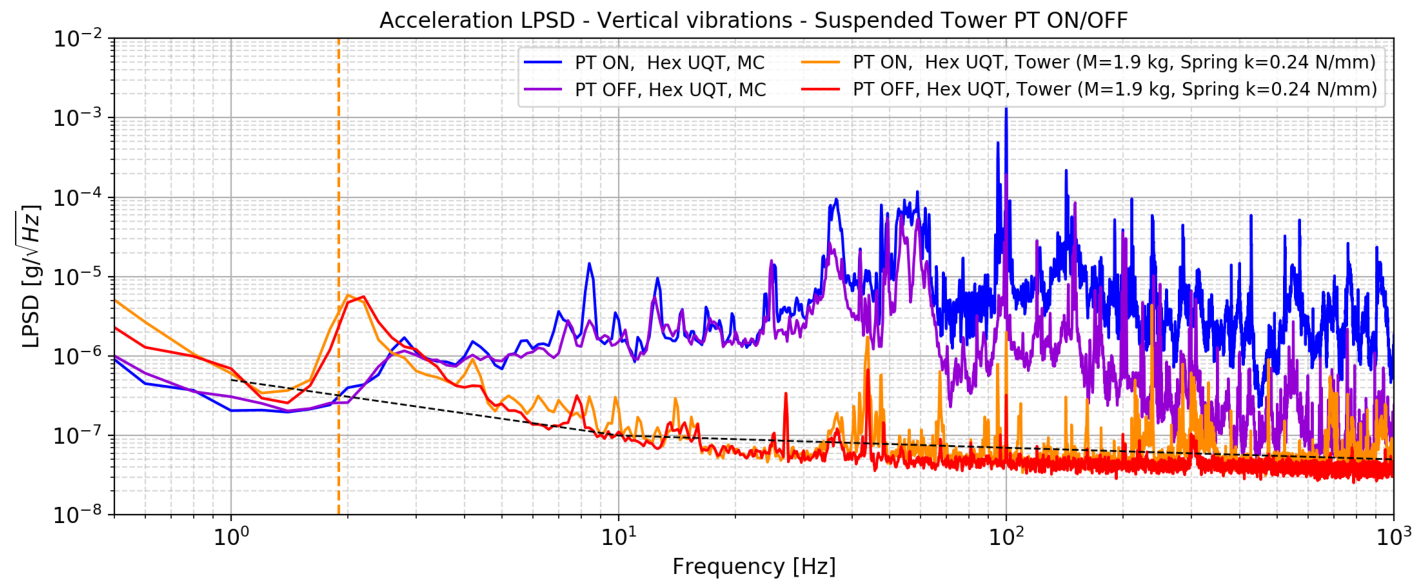
\includegraphics[width=\textwidth]{Figures/Experiment/vibration_vertical.pdf}
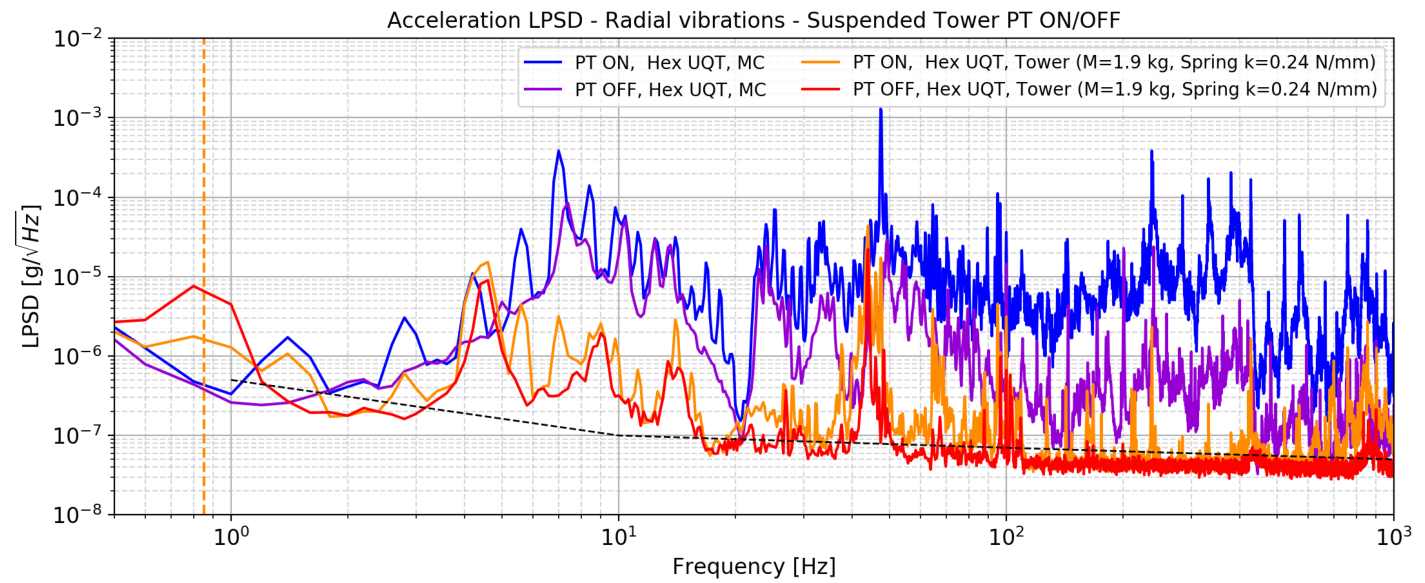
\includegraphics[width=\textwidth]{Figures/Experiment/vibration_radial.pdf}
\caption{Comparison of the vertical (top subplot) and radial (bottom subplot) vibration levels of the MC plate and the suspended tower in both PT ON and OFF configurations. The dashed black line is the accelerometer sensitivity, and the orange vertical dashed lines represent the position of the natural frequencies of the suspended tower derived from equations \ref{eq:Freq-Vertical} and \ref{eq:Freq-Radial}.}
\label{fig:vibration-levels}
\end{figure}
%  Figures taken from~\cite{Maisonobe:2018tbq}.

The main differences observed between these two PT configurations are coming from few pick-up lines which are mostly at high frequencies and arise from the acoustic noise generating by the operation of the pulse-tube cooling cycle.
At low frequencies ($<\SI{40}{\Hz}$), in the detector bandwidth, the impact of turning the PT ON is very small on the suspended tower, merely being expressed as resonance peaks of low amplitude.
As a matter of fact, by comparing the vibration level of the MC plate at PT OFF case (purple solid line) to the level of the suspended tower at PT ON case (orange solid line), one can further conclude that the suspended tower is not only efficient at reducing the PT-induced noises but also most of the whole setup-related vibrations from the building, the cryostat holding structure, and so on.
this demonstrate that vibration-wise, our detectors are largely insensitive to their surrounding environment, suggesting that they should run in optimal conditions inside the IP2I cryostat.

% Noise level for RED10
This optimal operations condition can be check by comparing the noise level affecting the signal measurement of a detector either installed on the mixing chamber plate or in the suspended tower. In this paragraph, this comparison is made with the \SI{200}{\g} detector RED10 whose heat channel is later characterized in the chapter \ref{ChapterEthem}. With a heat sensitivity of about \SI{100}{\nano\volt\per\kilo\eV} at around \SI{18}{\milli\kelvin}, RED10 is sensitive to perturbative displacements and vibrations. 

The noise levels are presented as LPSD expressed in \si{\volt\per\sqrthz}. These LPSD were measured as presented in the paragraph \ref{par:ethem-noise} dedicated to the characterization of the electronics noise affecting the heat channel of the bolometers.

Figurec \ref{fig:red10-vibration} shows the LPSDs obtained for RED10 on the MC plate as dashed lines, and on the suspended tower as solid lines. The \SI{1}{\volt} normalized heat signal template power spectrum and the theoretical noise calculations based on the full electro-thermal modeling of the detectors (see Sec.~\ref{sec:ethem-noise}) are also plotted as references. Measurements of the LPSDs were made with and without polarizing the NTD of RED10 in order to estimate the effect of the vibrations on the cabling, such as microphonics. Note that the discussion will mostly focus on the frequency range of interest, from \SI{1}{\Hz} to \SI{40}{\Hz}, as it corresponds to the detector signal bandwidth.

\begin{figure}
\centering 
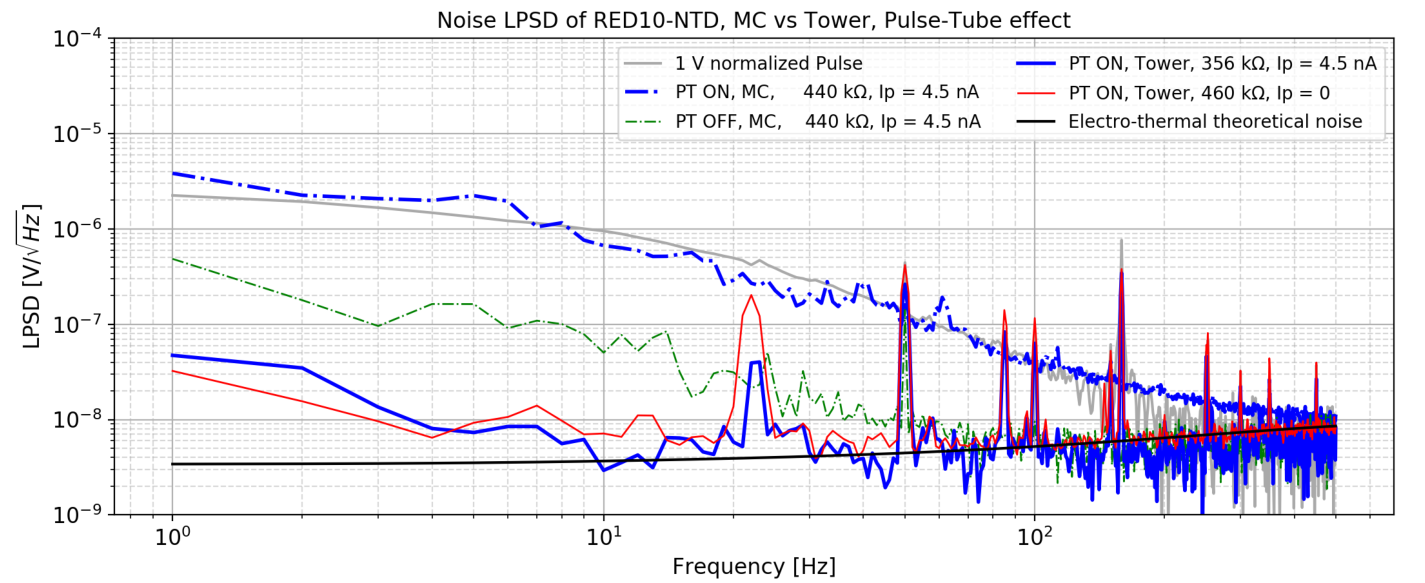
\includegraphics[width=\textwidth]{Figures/Experiment/red10_lspd_vibration.pdf}
\caption{Noise power spectra density for the NTD of RED10 mounted on the MC plate (dashed lines) and on the suspended tower (solid lines). Measurements were performed at optimal NTD polarization currents with PT ON and PT OFF at \SI{16}{\milli\kelvin}. The black solid line refers to the expected noise level derived from the electro-thermal model described in section \ref{sec:ethem-noise}, while the grey solid line shows the unit normalized pulse template illustrating the signal bandwidth.}
% Figures taken from~\cite{Maisonobe:2018tbq}.
\label{fig:red10-vibration}
\end{figure}


From comparing the various voltage PSD presented in Figure~\ref{fig:Noise-LPSD-RED2}, we can extract a few major conclusions regarding the effectiveness of the suspended tower at mitigating the vibration-induced noise on bolometers. 

The first obvious comparison is between the cases where the detectors are optimally polarized (blue curves) and either on the mixing chamber (dashed lines) or on the suspended tower (solid lines). The LPSD at the lowest frequencies is reduced by almost two orders of magnitude. 
Furthermore, we observe that the noise levels obtained PT ON and with the NTD optimally polarized (blue solid lines) are almost identical to the case where the NTDs are not polarized and the pulse-tube OFF (red dashed lines), suggesting that we are limited by both the electronics and the intrinsic thermal noise from the detector, and not by the vibrations when the detectors are mounted on the tower.
 This is confirmed by the fact that the resulting noise levels are very close to the theoretical expectations obtained with the electro-thermal model illustrated by the black solid lines.

Interestingly, we do not see on any of the three NTDs a \SI{1.8}{\Hz} pick-up noise as was potentially suggested from the vertical acceleration measurements shown as the red (PT OFF) and orange (PT ON) solid lines from Figure~\ref{fig:vibration-levels}. This  suggests that such frequency vibrations within the detector bandwidth do not limit the detector performance.

Finally, one can derive from Figure~\ref{fig:red10-vibration} that the noise PSD obtained with the NTDs optimally polarized on the suspended tower with PT ON (blue solid lines) are below the ones obtained with the detectors running on the mixing chamber with the PT OFF (green dashed lines). This observation confirm what was suggested from the vibration measurements shown in figure \ref{fig:red10-vibration}:  the suspended tower damps very efficiently the vibration-induced noise from the pulse-tube cryocooler, but makes the detectors insensitive to any residual vibrations from the surrounding environment of the experiment

The improvement on RED10 performances can be appreciated by computing its energy resolution. It was found that the heat resolution RED10 from \SI{14}{\kilo\eV} when installed on the mixing chamber, to \SI{400}{\eV}  when installed in the suspended tower. This impressive gain of almost two order of magnitude on the energy resolution can be explained by the detector RED10 being especially susceptible to vibrations. This detector would have been discarded due to poor performances without this internal mitigation solution.

%\footnote{Note that since this work, tremendous progress have been made on the low-noise cold cabling, the processing tools, and the low-energy calibration, such that RED10 actually achieved 50~eV (RMS) heat energy resolution later on, see Sec.~\ref{sec:randd-heatperformance}}.

Following the publication of this work~\cite{Maisonobe:2018tbq} similar improvement factors were found, between a factor of a few up to one order of magnitude, on all of the detector prototypes of the RED series.
The detectors operated at in the iP2I cryostats are no longer limited by vibrations, but only by the intrinsic JFET-based electronic noise limiting us from reaching the ultimate thermal fluctuation noise floor.
Based on this success, a new suspended tower
%shown in Fig.~\ref{fig:newtower}
that can host up to 5 RED detectors was installed in the IP2I cryostat in early 2020.  Though a similar elastic pendulum approach would not be feasible in the \Ricochet{} cryostat for the CryoCube, a slightly different three-spring pendulum approach is currently being investigated  for optimal operation of the CryoCube detector  at ILL.

%%% Bonus
%% Other mitigation solutions
%Several approaches have been considered to mitigate vibrations in dry dilution refrigerators: CUORICINO~\cite{DAddabbo:2017efe, Pirro:2006mu}, CUORE and its 988 TeO$_2$ detector array~\cite{Ligi:2016ldu,Santone:2017tjm}, and more recently the LUMINEU and CUPID-Mo collaborations with their three springs detector towers each hosting three to four crystals in the EDELWEISS cryostat in Modane~\cite{Armengaud:2017hit}. The CUORE experiment has implemented a different strategy. A Y-Beam (with three connecting points) at 300~K, isolated from the cryostat through \emph{Minus-K} suspensions, supports the whole 988 TeO2 detector array. Despite the use of three CRYOMECH PT415 pulse tubes, they report keV-scale detector energy resolutions \cite{Ligi:2016ldu,Santone:2017tjm}. Other implementations of passive decoupling systems on DDR, with a large panel of physics applications, can be found in \cite{Pelliccione:2012wx,Haan:2013iwa}.

%\cite{Olivieri:2017lqz}
%This suspended tower design reduces detector vibrations at the sub-$\mu$g/$\sqrt{\text{Hz}}$ level, with displacements in the order of a few nanometers (RMS) in all three axes, leading to substantial gains in energy resolutions
%as demonstrated in Ref.~\cite{Maisonobe:2018tbq}. 


%----------------------------------------------------------------------------------------
%	PRINCIPLES BOLOMETERS
%----------------------------------------------------------------------------------------
\section{Cryogenic Particle Detectors}

\subsection{Semiconductor Crystals for Particle Detection and Discrimination}

The use of cryogenic semiconductor crystals has been pioneered by the direct dark matter  detection experiments searching for low-mass dark matter. 
A wide variety of crystal materials can be used, but in recent years the leading materials have been: CaWO$_4$ in CRESST
%\cite{Abdelhameed:2019hmk}
, Ge and Si in (Super)CDMS
%\cite{Agnese:2013ixa}
, and Ge in EDELWEISS
%\cite{Armengaud:2017rzu}
.

These crystalline detectors, also designated as bolometers, aim at measuring the heat signals, in the form of thermal or athermal phonons, induced by a particle interaction.
Several temperature sensing techniques exist, but the most widely and mature ones are the (low-impedance) Transition Edge Sensors (TES) and neutron transmutation dopped germanium (NTD-Ge) thermistors. In both cases, the heat increase is measured via a change in resistance which is either measured as a current or voltage drop at the front-end of the readout electronics.

While their operation at cryogenic temperatures $\mathcal{O}(100)\ \si{\milli\kelvin}$ is challenging and expensive, cryogenic detectors feature a precise energy measurement with excellent energy resolution and background rejection down to recoil energies of $\mathcal{O}(1)$ \si{\kilo\eV}.
Indeed, the specificity of these detectors based on semiconductor crystal lies in the simultaneous measurement of a second observable, such as ionisation in semiconductors (Ge, Si) or scintillation in scintillating crystals (CaWO$_4$). This allows for the discrimination of the electronic recoils, induced by the radioactive background from the nuclear recoils, potentially generated by dark matter candidates, as in both cases the ionization/scintillation yields vary with the recoiling particle type.

Similarly to these dark matter candidates, a neutrino interacting with an atom of the semiconductor crystal of the detector through the CENNS process results in a nuclear recoil, giving access to the discrimination of science/background signals.
For this reason, the RICOCHET experiment aims at adapting this technology, in particular the germanium detectors of EDELWEISS, for the precise measurement of the CENNS process with the development of the CRYOCUBE detector array.


\subsection{Working Principle of Cryogenic Germanium Bolometers}

This work is focused on cryogenic germanium bolometers equipped with an ionization readout. Their working principles is illustrated with the scheme of figure \ref{fig:detector-principle}.

\begin{figure}
\centering
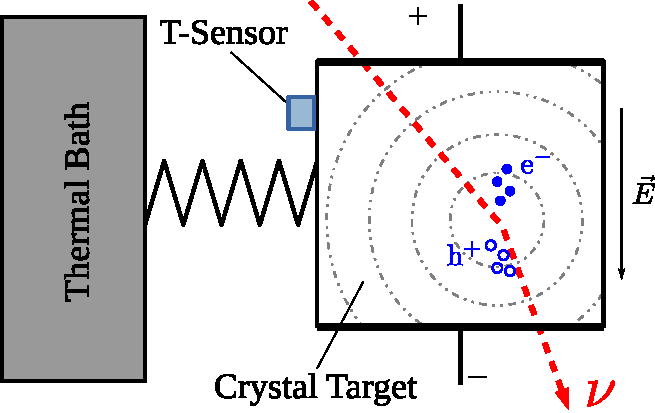
\includegraphics[scale=1]{Figures/Experiment/crystalline_detector_principle.pdf}
\caption{Working principle of a crystalline bolometer (here with additional charge-readout) for particle detection. The induced recoil from an interacting particle (here a nuclear recoil from an incident neutrino) on the atom of the germanium crystal release its recoil energy $E_R$ by creating phonons (illustrated as dashed concentric circles) and excited charge carriers (electron $e^-$ and holes $h^+$). The heat channel measures the increase in temperature $\Delta T$ from the phonons with a GeNTD thermal sensor. The ionization channel consists in the electrodes collecting the drifting charges by applying an electric field $\vec{E}$.
 Images adapted from \cite{Schumann:2019eaa}}
\label{fig:detector-principle}
\end{figure}

An ultra-pure semiconductor germanium crystal acts as an absorber: it is the element that serves as a target for the elastic collision of the incident particle. This interaction, called a recoil, deposits a recoil energy $E_R$ in the crystal which is expressed as thermal energy $E_{ph}$ as phonons and ionization energy $E_{e-h}$ as excited electron-hole pairs:
\begin{equation}
\label{energy}
E_R = E_{ph} + E_{Ion.}
\end{equation}

The fraction of the recoil energy going into the phonon and ionization energies is formalized with the quenching factor $Q$ such that:
\begin{equation}
\label{eq:quenching-intro}
E_{Ion.} = Q \cdot E_R \quad \textsf{and} \quad E_{ph} = (1-Q) \cdot E_R
\end{equation}
This quenching factor depends on the type of recoil induced by the incident particle interacting with the germanium crystal. The two major type of recoils considered in this work are the nuclear and the electronic recoils.
The electronic recoils (ER) are generated by incident photons or charged particles. In this case, the particle interacts with the electronic cloud of a germanium atom of the crystal. As a result, the entirety of the recoil energy $E_R$ is expressed in the excitation of the electrons, such that the associated quenching factor is $Q_{ER} = 1$ with $E_{Ion.} = E_R$.
The nuclear recoils (NR), induced by the CENNS process and neutrons, have the incident particle interacts with the nucleus of the atom. The transmitted recoil energy $E_R$ is immediately expressed as gain in momentum of the germanium nucleus. The movement of the nucleus generates vibrations of the crystal lattice, the phonons. The moving nucleus also disturbs the electronic cloud of its atom, thus creating some electron-hole pairs. The quenching factor $Q_{NR}$ associated with the nuclear recoils is an increasing function of the recoil energy $E_R$. It is comprised between 0 and 0.3 between 0 and \SI{20}{\kilo\eV}.
The intrinsic difference in heat and ionization energy between the nuclear and electronic recoils is the key aspect of the discrimination for the germanium detectors.

% Ionization Channel
The term ionization designates the creation of electron-hole pairs by a recoil. These excited charge carriers are the sole agents of the electric conduction in the semiconducting germanium, each carrying a positive or negative elementary charge $q_e = \SI{1.6e-19}{\coulomb}$.
The ionization energy $E_{e-h}$ determines the number $N_p$ of electron-hole pairs created in the crystal as:
\begin{equation}
E_{Ion.} = N_p \cdot \epsilon_{e^--h^+}
\end{equation}
with $\epsilon_{e^--h^+} \approx \SI{3}{\eV}$ the average energy of a pair in Germanium. 
Several electrodes applying an electric field $\vec{E}$ in the crystal will collect the drifting electrons and holes. The ionization signal is registered as voltage $\Delta V$ in Volt on the electrodes such that:
\begin{equation}
Q = N_p \cdot q_e = C_{el} \Delta V
\end{equation} 
with $Q$ the total collected electric charge in Coulomb and the $C_{el}$ the electric capacity of the electrode in Farad.
The ionization energy $E_{Ion.}$ is deduced from the measured voltage signal $\Delta V$:
\begin{equation}
E_{Ion.} = \frac{C_{el} \cdot \Delta V}{q_{e}} \cdot \epsilon_{e^--h^+}
\end{equation}
which is used to access the recoil energy $E_R$ with knowledge of the quenching in equation \ref{eq:quenching-intro}. This measure of the recoil energy through the ionization energy is defined as the ionization channel of the  detector.


% Phonons, Heat Channel
Phonons are vibrations of the crystal lattice which eventually thermalize with a global increase in temperature of the germanium crystal. The original thermal energy $E_{ph}$ is contained in the phonons created by the recoil and the recombination of the electron-hole pairs, such that $E_{ph} = E_R$.
% NL boost
Additional phonons are produced by the drifting the charge carriers across the crystal under the influence of the voltage bias $V_{bias}$ imposed by the electrodes. This process is the Neganov-Trofimov-Luke effect which can be considered as the equivalent of the Joule effect in semiconductors.
% \cite{Luke,Neganov:1985khw}
The boost to the thermal energy is defined as the Luke-Neganov energy expressed:
\begin{equation}
E_{NL} = N_p \cdot q_e \cdot V_{bias} = E_{Ion.} \frac{V_{bias}}{\epsilon_{e^--h^+}}
\end{equation}
Hence, the total thermal energy $E_{heat}$ induced by the recoil is expressed:
\begin{equation}
E_{heat} = E_{ph} + E_{NL} = E_R \left( 1 + Q \frac{V_{bias}}{\epsilon_{e^--h^+}} \right)
\end{equation}

It is linked to the increase in crystal temperature $\Delta T$ in Kelvin with the thermal capacity of germanium crystal $C_{Ge}$ in \si{\joule\per\kelvin} such that:
\begin{equation}
E_{heat} = C_{Ge} \cdot \Delta T
\end{equation}
% Thermal leakage
In time, the absorber cools down thanks to the thermal leakage, assured with gold wires between the detector and its copper chassis maintained at constant cryogenic temperature.
% thermistance
This thermal signal can be measured with a very sensitive thermometer. In this case, the thermal sensor is a Neutron-Dope Transmuted (NTD) germanium thermistor glued on the surface of the crystal. The electric resistance $R_{NTD}$ of this thermistance depends very strongly on its temperature $T_{NTD}$ following the law of Efros and Shllovskii \cite{mccammon}:
\begin{equation}
\label{eq:ntd-resistivity}
R_{NTD}(T_{NTD}) = R_0 \cdot \exp(\sqrt{\frac{T_0}{T_{NTD}}})
\end{equation}
where $R_0$ and $T_0$ are a characteristic resistance $\mathcal{O}(1)\ \si{\ohm}$ and temperature $\mathcal{O}(1)\ \si{\kelvin}$ of the NTD used. They depend on the geometry of the NTD, its doping, and the external constraints applied to it. 
Although this thermistor is made of germanium, it is doped and its physical properties are changed: it is conductive and thus has a free electron system in addition to a phonon system. The phonon system has a thermal capacity evolving like the cube of the temperature as the absorber (low thermal capacity), while the capacity of the electron system is linear with the temperature (high thermal capacity). We can therefore understand the usefulness of having an absorber-sensor couple: one serves as a target for the deposition of energy with low thermal capacity, while the other allows the measurement of the temperature rise through the epoxy glue assuring the thermal coupling such that $T_{NTD} \simeq T$.
Therefore, the GeNTD allows the measurement of temperature variations of the germanium crystal with its decreases in resistivity.
% Polarization
This $R_{NTD}$ resistivity is measured with the polarization of the NTD: a constant direct current $I$ of a few \si{\nano\ampere} is applied to the  thermistance. The Ohm's law gives:
\begin{equation}
V_{NTD} = R_{NTD} \cdot I
\end{equation}
so that the resistance is deduced from its measured voltage $V_{NTD}$.

% Cryogenic temperature
Cryogenic temperatures are necessary to be in a temperature range where the NTD thermistor becomes sufficiently sensitive to temperature variations. The exponential relation \ref{eq:ntd-resistivity} allows to obtain the largest variation of voltage $\Delta V_{NTD}$ for a small temperature variation $\Delta T$ at the lowest temperature of the detector $T$.
In the end, the heat energy $E_{heat}$ is derived from the measured voltage signal $\Delta V_{NTD}$ as:
\begin{equation}
E_{heat} = C_{Ge} \cdot I \cdot
\left. \frac{\mathrm{d}R_{NTD}}{\mathrm{d}T} \right|_{T}
\cdot
\Delta T
\end{equation}
It used to calculate the recoil energy $E_R$ with knowledge of the quenching $Q$ in equation \ref{eq:quenching-intro}. This measure of the recoil energy through the heat energy is defined as the heat channel of the detector.

% Discrimination
In the end, the cryogenic germanium detectors studied in this work have a double measurement of the recoil energy: the heat channel and the ionization channel. The double read-out is used to discriminate background-induced electron recoils from potential CENNS-induced nuclear recoils on an event-by-event basis.

\begin{figure}
\centering
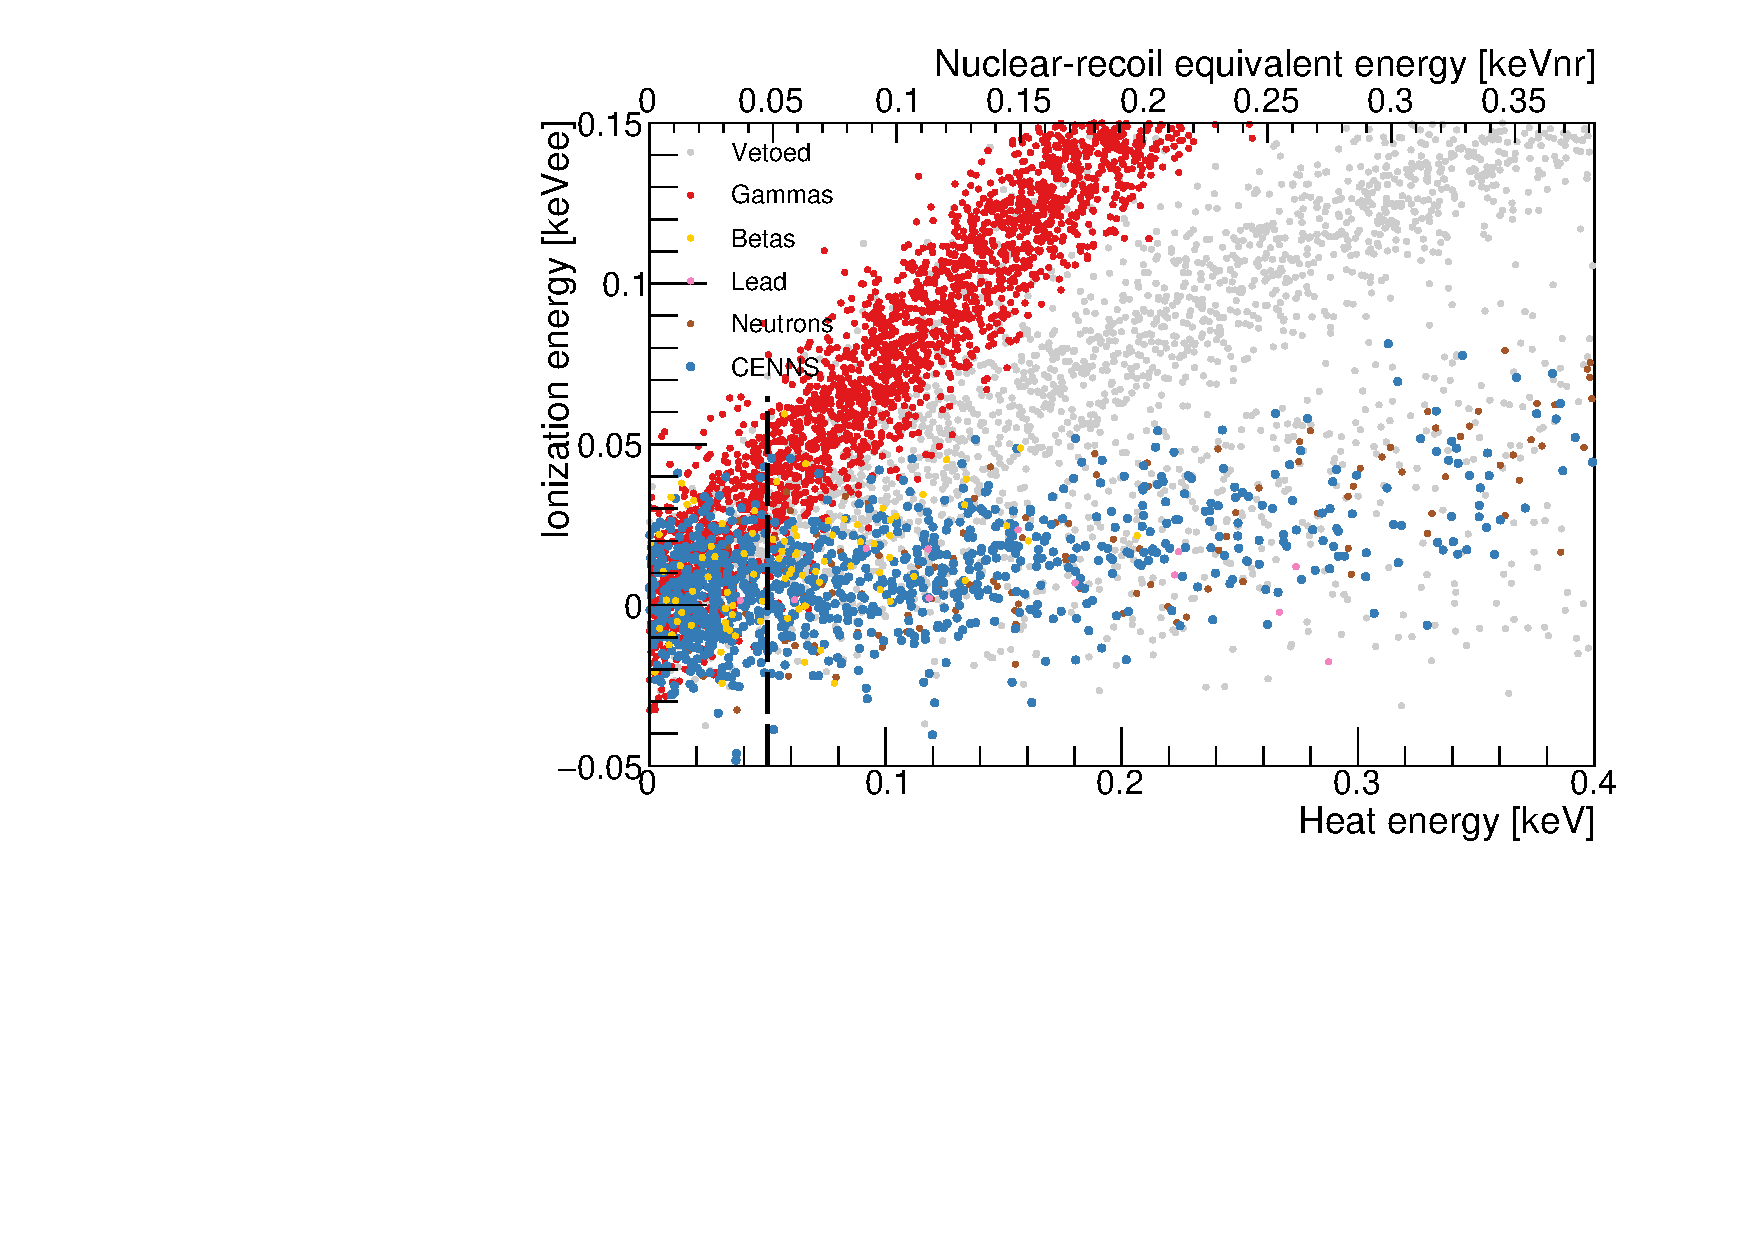
\includegraphics [width=0.7\textwidth]{Figures/Experiment/discrimination_simulation.pdf}
\caption{Illustration of the discrimination of simulated nuclear (blue) and electronic (red) recoils thanks to the simultaneous double-energy measurement with the ionization and heat channels  of the CRYOCUBE detectors. Other type of recoils with negligible event rate are also visible.}
\label{fig:discrimination-simulation}
\end{figure}

An illustration of this discrimination is displayed in figure \ref{fig:discrimination-simulation}. The graphic consists in the ionization energy $E_{Ion.}$ versus the heat energy $E_{heat}$ of simulated recoils of different types. Due to there difference in quenching factor $Q_{NR} < Q_{ER}$, the electronic recoils form the red band which is easily separated from the blue band of the nuclear recoils at sufficiently high energy (here for $E_{heat} \geq \SI{0.1}{\kilo\eV}$).  

Hence, the combination of the heat and ionization energies allows a highly efficient rejection of the dominant gamma backgrounds as well as the majority of beta-backgrounds. It is worth highlighting  that, in addition to the event-by-event discrimination, the simultaneous heat and ionization energy measurements also provides a direct measurement of the true nuclear recoil energy, hence avoiding any assumptions on the quenching factor $Q$ to be made. 

%This double-measurement design in a cryogenic bolometer is a characteristic of the EDELWEISS experiment and will be in use for RICOCHET.



\subsection{RED Prototype Detectors}

% RED series of detectoes
This thesis is inscribed in the R\&D program for the development of the detectors of the CRYOCUBE array. In order to meet its specification presented in paragraph \ref{par:cryocube}, the modelization of the detectors and the subsequent optimization of their design are tested and validated with experimental measurements in the IP2I R\&D cryostat.
These studies are carried out in collaboration with the EDELWEISS collaboration with the operation of the RED detector series. The RED series are R\&D-focused bolometers aiming at a full understanding and optimization of the heat and ionization channel. Eventually, the prototypes become very similar to the future element of the CRYOCUBE detector. All of the bolometers discussed hereafter in this work were fabricated by our collaborators at IJCLab, CEA Saclay, and Institut Néel. 

% Crystal shapeand weight
A RED prototype detector is based on cylindrical high-purity Ge crystal weighting between \SI{32}{\g} and \SI{200}{\g}. The crystal is maintained in a copper chassis with Teflon clamps whose heat conduction is negligible compared to the thermal leakage. Every RED detector has a heat channel consisting in one GeNTD thermal sensor glued on the surface of the crystal with gold wires assuring the electric cabling of the NTD and the thermal leakage of the whole detector. 

% Heat Only
In particular, early R\&D detectors such as RED10 and RED20, studied in the chapter \ref{ChapterEthem} were assembled with a very simple and clear design and do not possess an ionization channel. This permits to test thermal models and to better understand the physical processes involved in the thermal response of the detector.

% Electrodes and Ionization channel
Only the most recent RED prototypes, such as RED80 and REDN1 studied in the Chapter \ref{ChapterElectrodesExperimental} are equipped with an ionization channel.
The electrodes of these RED detectors are made by evaporating aluminium on the surface of the target material with various shape. It is possible to shape the electric field in the crystal with more complex designs of electrodes. In particular, the design FID38, studied in the chapter \ref{ChapterElectrodes} and inspired by the FID detectors of EDELWEISS-III, has two main collecting electrodes and two auxiliary veto electrodes allowing the tagging of surface events.



% In RED detectors, an energy deposit $\Delta E \sim \si{\kilo\eV}$ induces a temperature variation of the order of \si{\micro\kelvin} and leads to tensions measured from a few hundred \si{\nano\volt}. In practice, the heat signal is modeled by decaying exponential pulses with several characteristics times associated with the different thermalization processes and calorific capacities.


\subsection{Calibration Sources}
\label{par:calibration-source}
% Calibration source
The detectors are calibrated with particles inducing recoils of known heat $E_{heat}$ and the ionization $E_{Ion.}$ energies.
% Cosmic muons
For the first RED detectors, cosmic muons of high energy were used as calibration source. This natural source, available due to the very low overburden of the cryogenic facility, would generates a peak of electronic recoils centered on $E_R =  \SI{18}{\mega\eV}$. This calibration source has significant uncertainty on the position of the peak due to the wide cosmic muon energy distribution. Also, due to the non-linearity of the heat response, the measurements at low energies are severely underestimated with this calibration at high energy.

% Iron source
The muon calibration was quickly replaced with the use of radioactive iron sources.
An $^{55}$Fe calibration source was glued on the inner part of the detector's copper housing and facing the crystal surface opposite to the side on which is glued the Ge-NTD. It generates electronic recoils from a doublet peak of x-ray emission at \SI{5.90}{\kilo\eV} and \SI{6.49}{\kilo\eV}. This calibration method was mainly used for the operation of the RED detectors equipped solely with a heat channel (RED10 and RED20 in this work).

% activated germanium
The newest and most advantageous calibration method used in the current runs at the IP2I is based on the activation of the $^{71}$Ge in the crystal of the detectors with thermal neutrons. The detectors are activated with an intense AmBe neutron source. As such, the germanium crystal acts as a radioactive source generating electronics recoils from the x-ray emission of the K/L/M shells of the germanium. This peaks are located at the recoils energies of \SI{10.37}{\kilo\eV}, \SI{1.3}{\kilo\eV} and \SI{160}{\eV} respectively. All these calibrations peaks are in the exact energy range for the CENNS signal search $\mathcal{O}(1)$\si{\kilo\eV} while yielding a uniform distribution of the recoils on the whole volume of the detector. A direct application of this property is the experimental estimation of the fiducial volume and efficiency of the RED detectors as described in the chapter \ref{ChapterElectrodesExperimental}.


%----------------------------------------------------------------------------------------
%	BONUS UNUSED
%----------------------------------------------------------------------------------------

%\section{Detector principle}
%
%\begin{equation}
%\begin{cases}
%Q = Q_{ER} = 1 \\
%E_{Ion.}^{bulk} = Q \cdot E_R = E_R \\
%E_{heat} 
%=
%E_R 
%\cdot
%\frac{
%1 + Q_{ER}\frac{V_{bias}}{\epsilon_{e^--h^+}}
%}{
%1 + \frac{V_{bias}{\epsilon_{e^--h^+}}
%}
%= E_R
%\end{cases}
%\end{equation}
%
%\begin{equation}
%\begin{cases}
%Q = Q_{NR} \left( E_R \right) \\
%E_{Ion.}^{bulk} = Q_{NR}\left( E_R \right) \cdot E_R \\
%E_{heat} 
%=
%E_R 
%\cdot
%\frac{
%1 + Q_{NR} \left( E_R \right)\frac{V_{bias}}{\epsilon_{e^--h^+}}
%}{
%1 + \frac{V_{bias}{\epsilon_{e^--h^+}}
%}
%\end{cases}
%\end{equation}
%
%\begin{equation}
%\begin{cases}
%Q = Q_{HO} = 0 \\
%E_{Ion.}^{bulk} = Q_{NHO} \cdot E_R = 0 \\
%E_{heat} 
%=
%E_R 
%\cdot
%\frac{
%1 + Q_{HO} \left( E_R \right)\frac{V_{bias}}{\epsilon_{e^--h^+}}
%}{
%1 + \frac{V_{bias}{\epsilon_{e^--h^+}}
%}
%=
%E_R 
%\cdot
%\frac{
%1
%}{
%1 + \frac{V_{bias}{\epsilon_{e^--h^+}}
%}
%\end{cases}
%\end{equation}
